\chapter{RF PCB Design}
    \section{RF Principle}
        \begin{figure}[h]
            \centering
            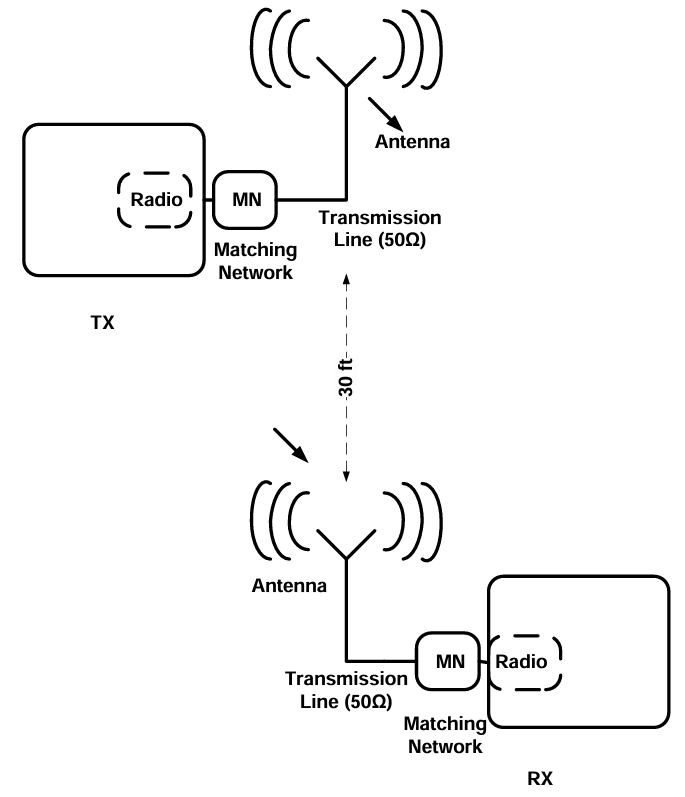
\includegraphics[width=0.5\textwidth]{figures/wireless_system.png}
            \caption{Typical Short-Range Wireless System}
            \label{fig:wireless_system}
        \end{figure}
        \newpage

        Về cơ bản, antenna là một dây dẫn lộ ra ngoài không gian. Nếu một dây dẫn có một tỉ lệ nhất định,
        hoặc là bội số bước sóng của tín hiệu\footnote{Harmonic antenna operation}, dây dẫn đó sẽ trở thành một antenna.
        Đây là điều kiện \textit{cộng hưởng}, vì năng lượng điện cung cấp cho antenna được bức xạ vào không gian.\cite{Infineon2023_rflayout}\par
        \begin{figure}[h]
            \centering
            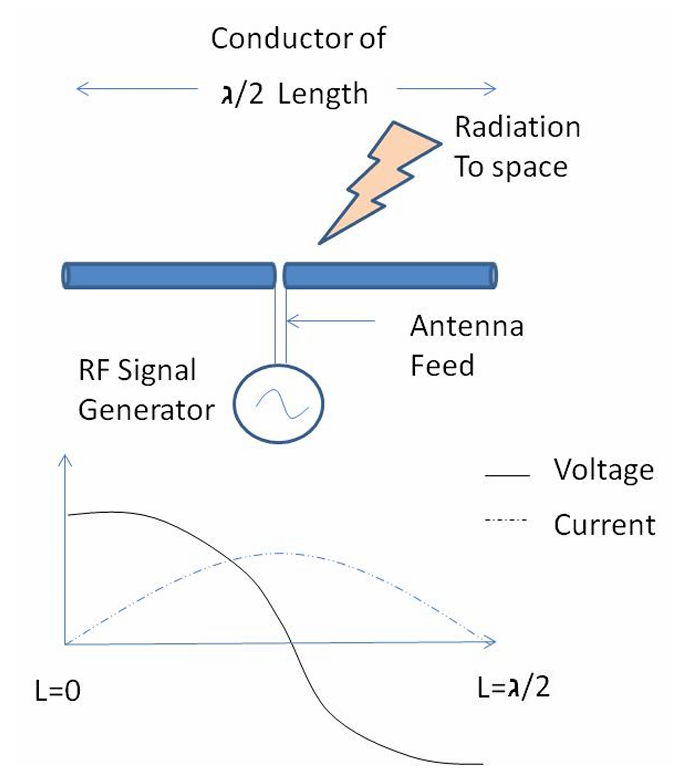
\includegraphics[width=0.5\textwidth]{figures/dipole_antenna_basic.png}
            \caption{Dipole Antenna Basic}
            \label{fig:dipole_antenna_basic}
        \end{figure}

        Trong \autoref{fig:dipole_antenna_basic}, dây dẫn có độ dài $\frac{\lambda}{2}$,
        trong đó $\lambda$ là bước sóng của tín hiệu điện.
        Nguồn phát tín hiệu cung cấp cho antenna tại điểm trung tâm
        bằng một transmission line, gọi là \textit{antenna feed}.
        Ở chiều dài này, sóng dừng điện áp và dòng điện hình thành
        trên toàn bộ chiều dài dây dẫn.\par

        \begin{figure}[h]
            \centering
            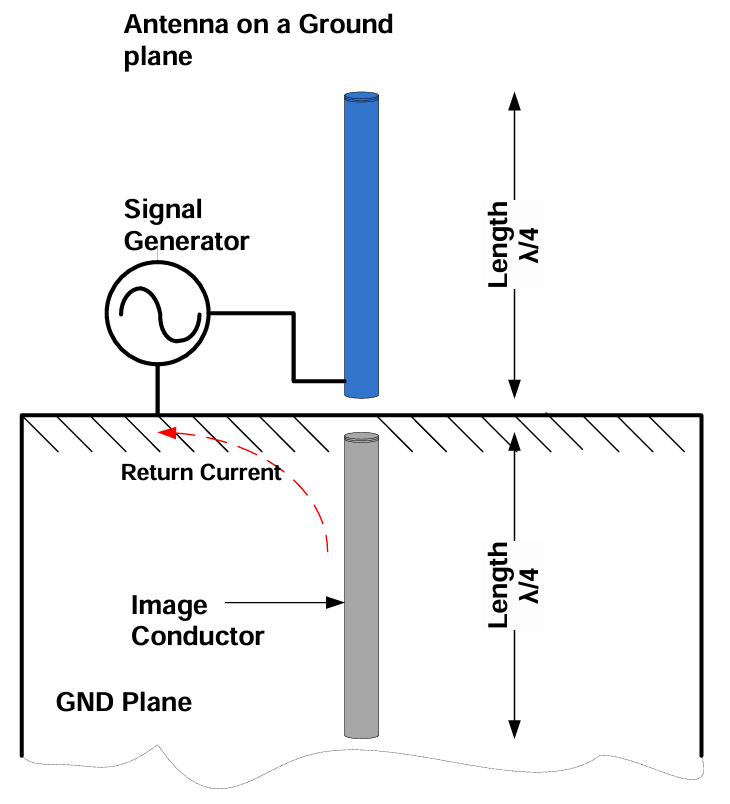
\includegraphics[width=0.35\textwidth]{figures/quarter_wave_antanna.png}
            \caption{Quarter-Wave Antenna}
            \label{fig:quarter_wave_antanna}
        \end{figure}

        Trong PCB, các mạch antenna có thể đạt được hiệu suất tương tự
        bằng cách thiết dây dẫn có chiều dài $\frac{\lambda}{4}$ bằng cách cụ thể như \autoref{fig:quarter_wave_antanna}.\par

        Bằng cách tạo ra một GND plan ở một khoảng cách nhất định bên dưới dây dẫn,
        một hình ảnh phản chiếu được tạo ra có cùng độ dài $\frac{\lambda}{4}$,
        khi kết hợp lại, nó hoạt động giống như một antenna lưỡng cực.
        Thiết kế antenna này được gọi là \textbf{quarter-wave monopole antenna} (antenna đơn cực một phần tư bước sóng).
        Tín hiệu được truyền trên một đường dẫn single-ended và GND plan hoạt động như một đường hồi tiếp.\par
    
    \section{Các loại antenna}
        \subsection{Wire antenna}
        \subsection{PCB antenna}
        \subsection{Chip antenna}

    \section{Thông số antenna}
        \begin{figure}[h]
            \centering
            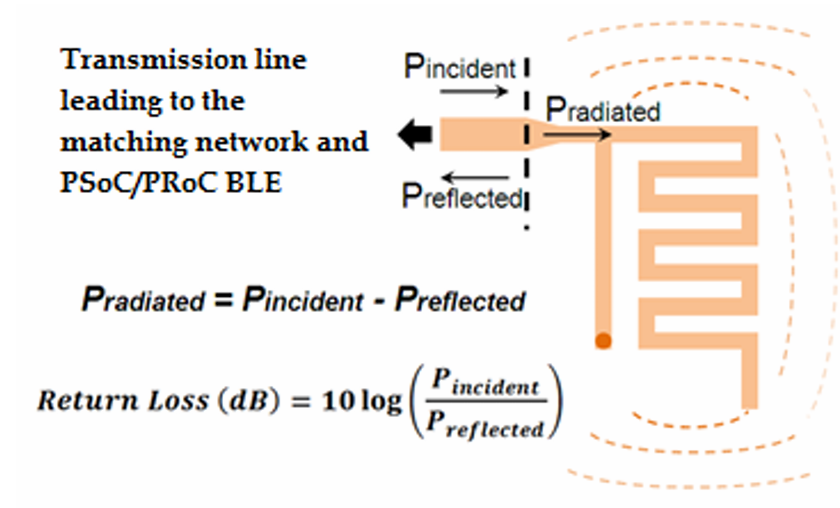
\includegraphics[width=0.5\textwidth]{figures/return_loss_antenna.png}
            \caption{Return Loss}
            \label{fig:return_loss_antenna}
        \end{figure}

        
        \begin{table}[h]
            \centering
            \begin{tabular}{|c|c|c|c|}
                \hline
                \rowcolor{TLgreen!50}
                &   &   &   \\
                \arrayrulecolor{TLgreen!50}
                \cline{1-4}
                \arrayrulecolor{black}
                \multirow{-2}{*}{\cellcolor{TLgreen!50}$\mathbf{S_{11}}$}  &   \multirow{-2}{*}{\cellcolor{TLgreen!50}\textbf{Return Loss (dB)}}  &   \multirow{-2}{*}{\cellcolor{TLgreen!50}\textbf{$\mathbf{\frac{P_{reflected}}{P_{incident}}}$ (\%)}}    &   \multirow{-2}{*}{\cellcolor{TLgreen!50}\textbf{$\mathbf{\frac{P_{radiated}}{P_{incident}}}$ (\%)}} \\\hline
                -20 &   20 &   1\%  &   99\% \\\hline
                -10 &   10 &   10\% &   90\% \\\hline
                -3  &   3  &   50\% &   50\% \\\hline
                -1  &   1  &   79\% &   21\% \\\hline
            \end{tabular}
            \caption{Return Loss and Power Reflected from Antenna}
            \label{tab:return_loss_antenna}
        \end{table}